\documentclass[11pt,a4paper]{article}
\usepackage[utf8]{inputenc}\usepackage[T1]{fontenc}
\usepackage[margin=1in]{geometry}
\usepackage{amsmath,amssymb,booktabs,graphicx,enumitem,xcolor,parskip,titlesec}
\usepackage[hidelinks]{hyperref}
\graphicspath{{figures/}}
\definecolor{qnavy}{RGB}{20,40,75}\definecolor{qgrey}{RGB}{90,90,90}\definecolor{qred}{RGB}{150,30,30}
\titleformat{\section}{\large\bfseries\color{qnavy}}{\thesection}{0.6em}{}
\begin{document}\thispagestyle{empty}
\noindent
{\large\bfseries\color{qnavy} Report R16 --- A Plan Written Blind, Then Executed}\\[2pt]
{\color{qgrey}ACRIN 6668 sealed holdout. An isolated agent wrote the analysis from schema alone;
the plan was hashed before any outcome was read; the verdict is CONFIRMED.}\\[6pt]
{\color{qgrey}\rule{\textwidth}{0.4pt}}

\medskip
\noindent 16 August 2026 \quad\textbullet\quad Quantara

\section*{Summary}

This is the second cohort for the autonomous-generation arm, and the first run of a
\emph{structurally} separated generator. An agent whose entire readable surface was one
JSON file --- form names, column names, row counts and the trial's data dictionary, with no cell
value from any outcome field --- wrote a 493-line pre-registered analysis plan for a cohort it had
never seen. The plan was SHA-256 hashed at
\texttt{752b7462fce56899\ldots cb74e6770} on 15 August at 13:07:14\,Z, before the coordinator
read a single outcome value. It was then executed as written.

\textbf{Verdict: CONFIRMED.} Higher post-treatment FDG peak SUV predicts shorter overall survival:
\textbf{HR 1.202 per doubling} (95\% CI 1.100--1.315), permutation $p = 0.0005$, on 166 analysed
patients with 125 events. That is the association ACRIN 6668 was designed to test, recovered by a
plan written in ignorance of the data's contents.

All nine integrity gates passed. Three of four positive controls corroborated, the fourth
declared uninformative by its own pre-registered rule rather than quietly dropped. All seven
pre-declared robustness tests agree in direction and survive Holm correction.

\section{What the generator produced, and what it caught}

The plan is in \texttt{evidence/PLAN\_hashed\_752b7462.yaml}. From schema and dictionary alone it
identified twelve traps in advance. Four mattered:

\begin{itemize}[leftmargin=1.3em,itemsep=2pt]
\item \textbf{Immortal time.} The exposure is measured 8--20 weeks after chemoradiotherapy, so
      measuring survival from registration would guarantee survival to exposure. The plan set the
      time origin at the post-treatment PET (a landmark) and made $\min(T) \geq 0$ a gate.
\item \textbf{Vital-status code 9} means ``dead, date of death unknown''. The obvious
      \texttt{event = (f1e2 == 2)} silently undercounts deaths. The plan treated 9 as an event and
      made a censoring sensitivity a \emph{condition} of confirming.
\item \textbf{Cutoff forking.} Form SS carries 1{,}185 rows keyed by an SUV inclusion cutoff ---
      five analyses per patient, a ready-made garden of forking paths. The plan locked SS to the
      single most inclusive cutoff and forbade any comparison across cutoffs.
\item \textbf{Undocumented uniqueness.} The recon package did not state that form LE is one row
      per patient, yet the primary exposure depended on it. The plan required verification and
      pre-specified a duplicate-resolution rule.
\end{itemize}

That last one fired: LE has 244 rows over 243 patients. The plan's rule resolved it and reported
the single affected patient.

\section{Results}

\subsection{Gates}

\begin{center}
\begin{tabular}{@{}llr@{}}
\toprule
\textbf{Gate} & \textbf{Check} & \textbf{Result} \\
\midrule
G1 & two release samples recombine, disjoint, A0 = 251 rows / 251 patients & PASS \\
G2 & six join counts reproduced exactly; 0 orphans in any form & PASS \\
G2b & LE duplicates resolved by the declared rule (1 patient) & PASS \\
G3 & SS confirmed keyed by cutoff (values 0/2/2.5/3/3.5; modal 5 rows per patient) & PASS \\
G4 & no outcome-period leakage; exposure hash unchanged from the freeze & PASS \\
G5 & $251 = 166 + 85$, ledger reconciles exactly & PASS \\
G6 & permutation null centred (mean $z$ 0.034, SD 0.982, rejection 0.042) & PASS \\
G7 & exposure coverage $\geq 180$ (observed exactly 180) & PASS \\
G8 & vital-status tally: 125 dead, 38 alive, 3 lost; median follow-up 49.2 months & PASS \\
G9 & primary point estimate lies inside its own CI \emph{(added after a bug, \S5)} & PASS \\
\bottomrule
\end{tabular}
\end{center}

\subsection{Exclusion ledger}

\begin{center}
\begin{tabular}{@{}llr@{}}
\toprule
E2 & ineligible / duplicate registration & 18 \\
E3 & no radiotherapy commenced & 15 \\
E4 & no post-treatment PET timepoint (time origin undefined) & 38 \\
E5 & post-RT peak SUV missing & 10 \\
E8 & PET outside the 28--280 day post-RT window & \phantom{0}4 \\
\midrule
& E1, E6, E7 & \phantom{0}0 \\
\midrule
\textbf{Total excluded} & & \textbf{85} \\
\textbf{Analysed} & & \textbf{166} \\
\bottomrule
\end{tabular}
\end{center}

\subsection{Primary and controls}

\begin{center}
\begin{tabular}{@{}llrl@{}}
\toprule
& \textbf{Test} & \textbf{HR} & \textbf{Outcome} \\
\midrule
\textbf{Primary} & OS on log$_2$ post-RT peak SUV & \textbf{1.202} & perm.\ $p = 0.0005$ \\
& & & 95\% CI 1.100--1.315 \\
\midrule
PC0 & post-RT SUV below pre-RT (outcome-free) & --- & \textbf{PASS} (94.4\%) \\
PC1 & progression by day 365 $\rightarrow$ shorter OS & 2.463 & \textbf{PASS} ($p = 3.8\times10^{-5}$) \\
PC2 & performance status $\geq 1$ vs 0 & 1.382 & PASS-WEAK ($p = 0.072$) \\
PC3 & weight loss $\geq 5\%$ & --- & UNINFORMATIVE-BY-N (26 exposed) \\
\bottomrule
\end{tabular}
\end{center}

PC1 is the one that matters: it validates that the survival clock, the per-patient reduction over
6.3 follow-up rows per person, and the vital-status map were assembled correctly. Its near-tautological
clinical content is the point --- it fails if the plumbing is wrong.

PC2 came out in the right direction but short of significance, and PC3 was declared uninformative
because only 26 patients had $\geq 5\%$ weight loss against a pre-declared threshold of 30. The
plan had \emph{anticipated} both: trial eligibility screens performance status, so range
restriction was expected and given its own outcome branch in advance rather than being explained
afterwards.

\begin{center}
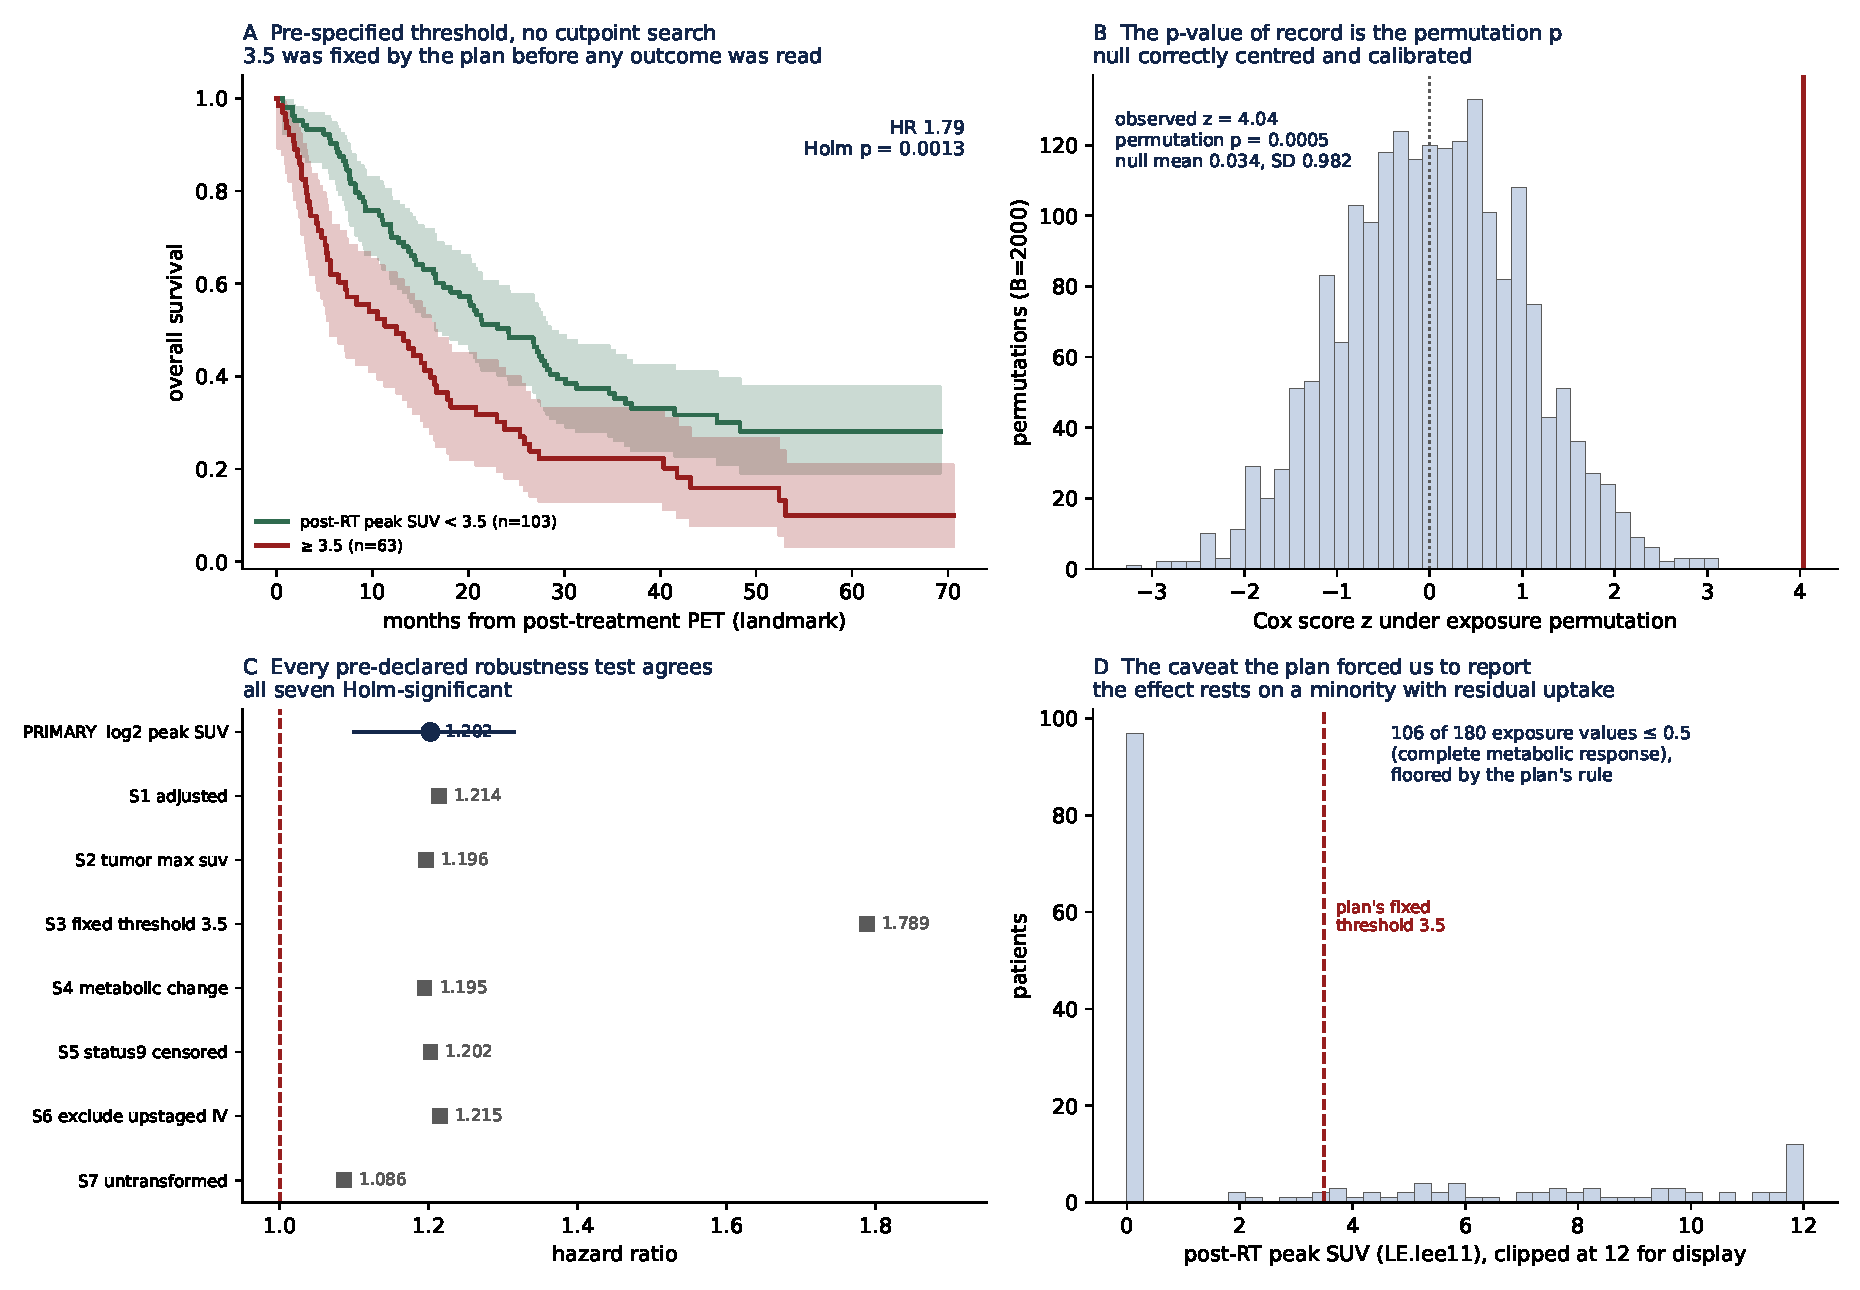
\includegraphics[width=\textwidth]{r16_panels.pdf}
\end{center}
\noindent{\small\color{qgrey}\textbf{A} Survival split at the plan's fixed 3.5 threshold --- no
cutpoint search was permitted. \textbf{B} The permutation null and the observed statistic.
\textbf{C} Primary and all seven robustness tests. \textbf{D} The exposure distribution, and the
caveat the plan forced into the open.}

\subsection{Robustness}

All seven pre-declared secondary tests, Holm-corrected across the family:

\begin{center}
\begin{tabular}{@{}llrrr@{}}
\toprule
& \textbf{Test} & \textbf{HR} & \textbf{Holm $p$} & \textbf{$n$} \\
\midrule
S1 & adjusted (age, sex, stage, performance status) & 1.214 & 0.0002 & 165 \\
S2 & tumour max SUV instead of peak & 1.196 & 0.0002 & 166 \\
S3 & fixed threshold 3.5 (no search) & 1.789 & 0.0013 & 166 \\
S4 & metabolic change, post minus pre on log$_2$ & 1.195 & 0.0002 & 165 \\
S5 & code-9 deaths censored instead of events & 1.202 & 0.0002 & 166 \\
S6 & excluding patients upstaged to IV & 1.215 & 0.0002 & 161 \\
S7 & untransformed SUV (per unit) & 1.086 & $<0.0001$ & 166 \\
\bottomrule
\end{tabular}
\end{center}

The adjusted estimate is slightly \emph{larger} than the unadjusted one, and the effect survives
excluding upstaged patients, changing the SUV field, and changing the transformation.

\section{The caveat the plan forced us to report}

\textbf{106 of 180 exposure values were at or below 0.5} --- complete metabolic response ---
and were floored by the plan's rule. So 59\% of the cohort sits at a single tied value and the
association is carried by the minority with residual uptake. The plan required this count to be
reported, which is why it appears here rather than in a reviewer's letter. S3, the binary split at
a fixed 3.5, is arguably the more interpretable form of the same finding: median survival is
clearly separated (Figure~A) with HR 1.79.

\section{Two coordinator errors, and one that gates did not catch}

Recorded because this report is partly about process, and the process failed in ways worth
knowing.

\textbf{Two implementation errors were mine, not the plan's.} First, I wrote LE uniqueness as a
hard stop when the plan had already anticipated the duplicate and specified a remedy --- the plan
had thought further ahead than my executor. Second, the landmark date came back empty because the
CSVs capitalise day-offset fields (\texttt{TAe7d}) differently from the dictionary the plan quotes
(\texttt{tae7d}); same field, different case. Neither required reinterpreting the plan.

\textbf{One error the gates did not catch.} An earlier execution reported the primary as
HR 1.382 with CI 1.050--1.124 --- a point estimate outside its own interval. Inside the control
blocks I had reused \texttt{hr} and \texttt{ci} as scratch names, clobbering the primary's values
before the verdict logic read them, so the verdict was briefly evaluated using PC2's hazard ratio.
All eight of the plan's gates passed while this was true. The conclusion survives correction, but
it was momentarily reached by accident.

What caught it was not a gate but an internally impossible number. Gate G9 was added afterwards to
assert that the primary point estimate lies inside its own confidence interval. \textbf{A
pre-registration protects against choosing your analysis after seeing results; it does not protect
against implementing it wrongly.} Those are different failure modes and need different defences.

\section{Limitations}

\textbf{Single trial, one modality, tabular only.} This used the core-lab PET assessments, not the
135.5\,GiB of PET/CT imaging. The generalisation claim concerns an unseen cohort and data shape,
not an unseen imaging pipeline.

\textbf{The exposure is 59\% floored} (\S4).

\textbf{Two of four controls did not fully corroborate.} PC2 weak, PC3 uninformative. Under the
plan's aggregate rule this is sufficient for CONFIRMED, because PC2 was in the right direction and
PC1 passed strongly --- but a fully corroborated run would have been stronger.

\textbf{G7 passed at exactly its threshold} (180 against $\geq 180$). One patient fewer and the
declared fallback chain would have fired, changing the exposure source.

\textbf{Not an independent replication of the trial.} The published ACRIN 6668 analysis used the
same data. The claim here is about the \emph{process} --- that a blind, pre-registered plan
recovers a known result --- not about establishing the biology afresh.

\section*{Reproducing this report}

\texttt{evidence/PLAN\_hashed\_752b7462.yaml} (the plan as hashed),
\texttt{evidence/PREREGISTRATION.json} (hash and timestamp),
\texttt{evidence/execute\_plan.py} (the executor),
\texttt{evidence/exposure\_table.csv} (frozen at Stage 1, SHA-256
\texttt{854378633ea6992c\ldots}), \texttt{evidence/analysis\_frame.csv},
\texttt{evidence/permutation\_z.npy} (all 2{,}000 null statistics),
\texttt{evidence/gates.json}, \texttt{evidence/results.json}. Figure:
\texttt{python3 make\_figure.py}.

\end{document}
